\chapter{Progettazione dell'applicazione}

\section{Architettura generale dell'applicazione}

"Dalla Ricetta Al Carrello" è un'applicazione desktop organizzata a livelli. \\
La separazione delle responsabilità evita che l'interfaccia grafica esegua direttamente query SQL e rende più semplice modificare una parte del sistema senza intervenire sulle altre. Il flusso ordinario è il seguente:

View → Controller → Service → DAO → MySQL

Le view (pacchetto \textbf{view}, realizzate in Swing) raccolgono gli input dell'utente e aggiornano le schermate.\\
I controller (pacchetto \textbf{controller}) espongono in modo sottile le operazioni richieste dall'interfaccia, senza contenere logica propria.\\
I service (pacchetto \textbf{service}) applicano le regole di dominio, calcolano i valori derivati e coordinano le transazioni.\\
I DAO (pacchetto \textbf{dao}) contengono il codice JDBC e traducono le righe del database negli oggetti del pacchetto model, che rappresentano le entità persistenti del dominio (utente, ricetta, ingrediente, ordine, categoria, promozione, sconto, recensione).

La finestra principale, \textbf{MainFrame}, utilizza un \textbf{CardLayout} per alternare tra la schermata di login/registrazione e la shell principale dell'applicazione (\textbf{ShellPanel}).\\
Dopo l'autenticazione, ShellPanel mostra una barra di navigazione laterale con le funzionalità disponibili; le voci visibili dipendono dal ruolo dell'utente autenticato (UTENTE o ADMIN), letto dalla colonna Ruolo di UTENTI.

Il database risiede in locale e viene raggiunto direttamente dall'applicazione: si tratta quindi di un'architettura desktop a due livelli (2-tier), senza un server applicativo intermedio.
\vspace{1em}

\textbf{Scelte progettuali principali:}
\begin{itemize}
    \item \textbf{Un DAO per ogni entità}. Ogni tabella dello schema fisico ha un'interfaccia DAO e una relativa implementazione JDBC, comprendente sempre le operazioni di inserimento, aggiornamento (dove previsto dalla specifica) e lettura. Questa uniformità rende immediato individuare dove risiede il codice di accesso a una determinata tabella.
    \item \textbf{Le query di aggregazione risiedono nei service, non nei DAO}. Le query con GROUP BY o che uniscono più tabelle a scopo statistico (classifiche, vantaggi attivi, viste amministrative) sono scritte come SQL incapsulato direttamente in metodi dei service, non nei DAO. Il criterio adottato è che un DAO risponde alla domanda "come leggo o scrivo questa singola entità", mentre un report attraversa più entità contemporaneamente e non è legato al ciclo di vita di nessuna di esse in particolare.
    \item \textbf{La connessione JDBC è sempre iniettata nel costruttore del DAO}, mai passata come parametro dei singoli metodi. Per le operazioni transazionali che coinvolgono più DAO (ad esempio la pubblicazione di una ricetta o la creazione di un ordine, che toccano più tabelle in un'unica unità atomica), il service crea più istanze di DAO passando loro la medesima Connection: condividendo lo stesso oggetto, tutte le operazioni fanno parte della stessa transazione. Questa impostazione rende uniforme la firma dei metodi dei DAO, indipendentemente dal fatto che vengano usati singolarmente o all'interno di una transazione più ampia.
    \item \textbf{La password non è mai gestita in chiaro lato Java}. L'hashing avviene interamente lato database tramite la funzione SHA2(?, 512) inclusa direttamente nella query di registrazione e di accesso: la password in chiaro viaggia solo come parametro JDBC per il tempo strettamente necessario, senza mai essere calcolata, confrontata o salvata in memoria come hash lato applicativo.
\end{itemize}

\vspace{1em}

\section{Gestione degli errori e validazione dell'input}

La validazione è distribuita su più livelli:
\begin{itemize}
    \item I form Swing controllano la presenza dei campi obbligatori e la validità dei formati (date, numeri) prima di inviare la richiesta al livello sottostante.
    \item Il database applica comunque i propri vincoli (chiavi esterne, \textbf{CHECK}, \textbf{UNIQUE}, trigger), che restano l'ultima linea di difesa anche in caso di validazione lato Java incompleta.
    \item I trigger SQL intervengono su casi specifici del dominio: ad esempio impediscono la creazione di un ordine se l'utente non ha impostato un indirizzo di spedizione, oppure impediscono la sovrapposizione di due sconti sulla stessa combinazione categoria/promozione.
\end{itemize}

Gli errori di accesso ai dati propagano una \textbf{SQLException}, gestita dalle view tramite messaggi in linea nell'interfaccia (etichette di stato colorate) o tramite finestre di dialogo (\textbf{JOptionPane}) per le operazioni più delicate, come l'esecuzione dell'operazione di rimozione utenti incoerenti, che richiede una conferma esplicita prima di procedere data la sua irreversibilità.

Un caso gestito con un'eccezione dedicata è quello dell'account disattivato: se un utente con credenziali corrette ma con \textit{Attivo = FALSE} prova ad accedere, il livello service intercetta il caso e lancia una \textbf{AccountDisattivatoException}, distinta da una semplice mancata corrispondenza delle credenziali. In questo modo la schermata di login può mostrare un messaggio specifico ("account disattivato, contatta l'assistenza") invece del generico "credenziali non valide".

Le operazioni che richiedono l'accesso al database — accesso, ricerche, pubblicazione di ricette, creazione di ordini, operazioni amministrative — vengono eseguite tramite \textbf{SwingWorker}: il codice JDBC gira su un thread separato da quello dell'interfaccia grafica (Event Dispatch Thread), così l'applicazione resta reattiva anche durante operazioni più lente, senza bloccare l'interfaccia durante l'attesa della risposta dal database.
\vspace{1em}

\section{Guida alle schermate}

Questa sezione descrive le principali schermate dell'applicazione nell'ordine in cui un utente le incontra normalmente, a scopo di documentazione visiva del lavoro svolto.

\subsection{Accesso e registrazione}

La schermata di apertura mostra un'unica card centrale, con due modalità alternabili tramite un collegamento testuale: accesso con email e password esistenti, oppure registrazione di un nuovo account (nome, cognome, email, password e indirizzo di spedizione facoltativo).\\
In entrambi i casi l'operazione è asincrona: il pulsante si disabilita durante l'elaborazione e un'etichetta di stato comunica l'esito.

\begin{figure}[H]
    \centering

    \begin{minipage}{0.48\textwidth}
        \centering
        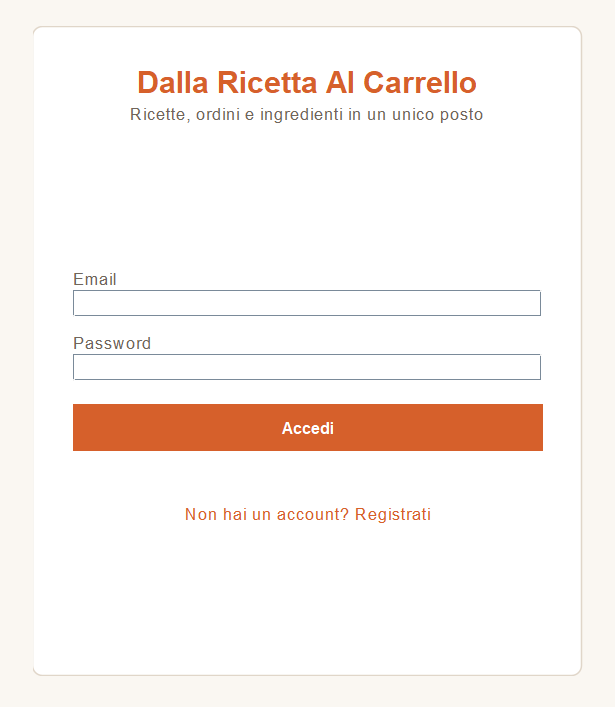
\includegraphics[width=\textwidth]{images/login.png}
        \caption{Schermata di login.}
        \label{fig:login}
    \end{minipage}
    \hfill
    \begin{minipage}{0.48\textwidth}
        \centering
        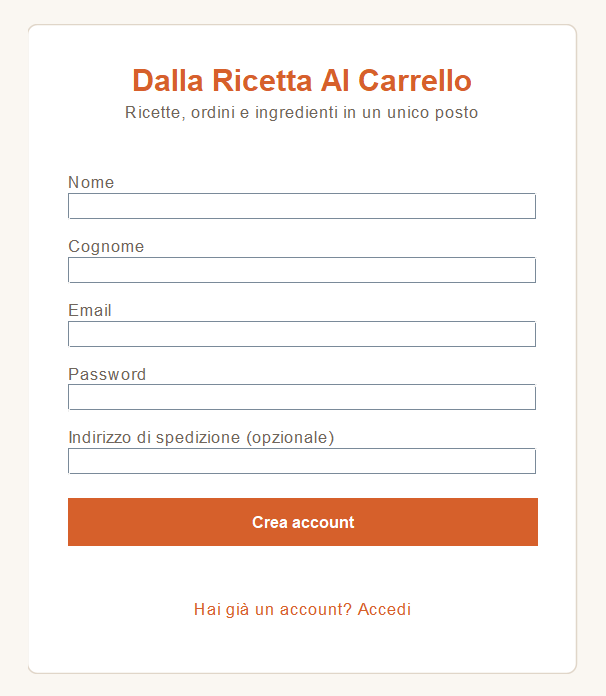
\includegraphics[width=\textwidth]{images/registrazione.png}
        \caption{Schermata di registrazione.}
        \label{fig:reg}
    \end{minipage}

\end{figure}

\subsection{Struttura post-accesso: barra di navigazione}

Dopo l'autenticazione, l'interfaccia si presenta con una barra laterale a sinistra (sfondo arancione per l'utente standard, blu/indaco per l'amministratore — colori volutamente diversi per rendere immediatamente riconoscibile il contesto) e un'area contenuti a destra, che cambia in base alla voce di menu selezionata.\\
In fondo alla barra laterale sono presenti il nome dell'utente autenticato e il pulsante di uscita.

\begin{figure}[H]
    \centering
    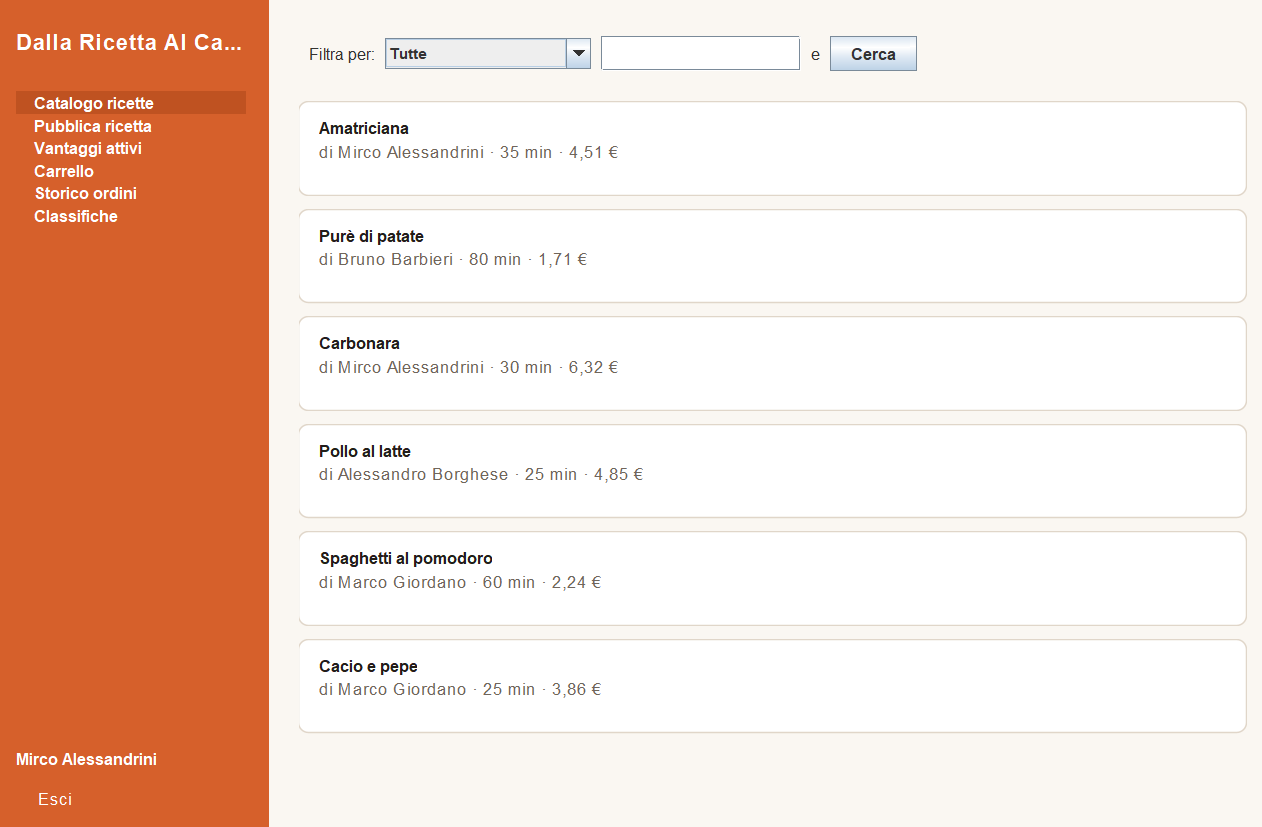
\includegraphics[width=1\textwidth]{images/menu.png}
    \caption{Schermata principale con menù di navigazione.}
    \label{fig:nav}
\end{figure}

\subsection{Catalogo ricette e dettaglio}

La sezione "Catalogo ricette" mostra l'elenco delle ricette disponibili, con un pannello di filtro che permette di cercare per nome, ingrediente, tempo massimo di preparazione, fascia di prezzo, autore o categoria.\\
Selezionando una ricetta si accede al dettaglio: ingredienti in elenco con relative quantità, testo della preparazione, categorie di appartenenza mostrate come etichette colorate, una card per aggiungere la ricetta al carrello con selezione della quantità, e una card per pubblicare una recensione (voto da 1 a 10 e commento facoltativo).

\begin{figure}[H]
    \centering
    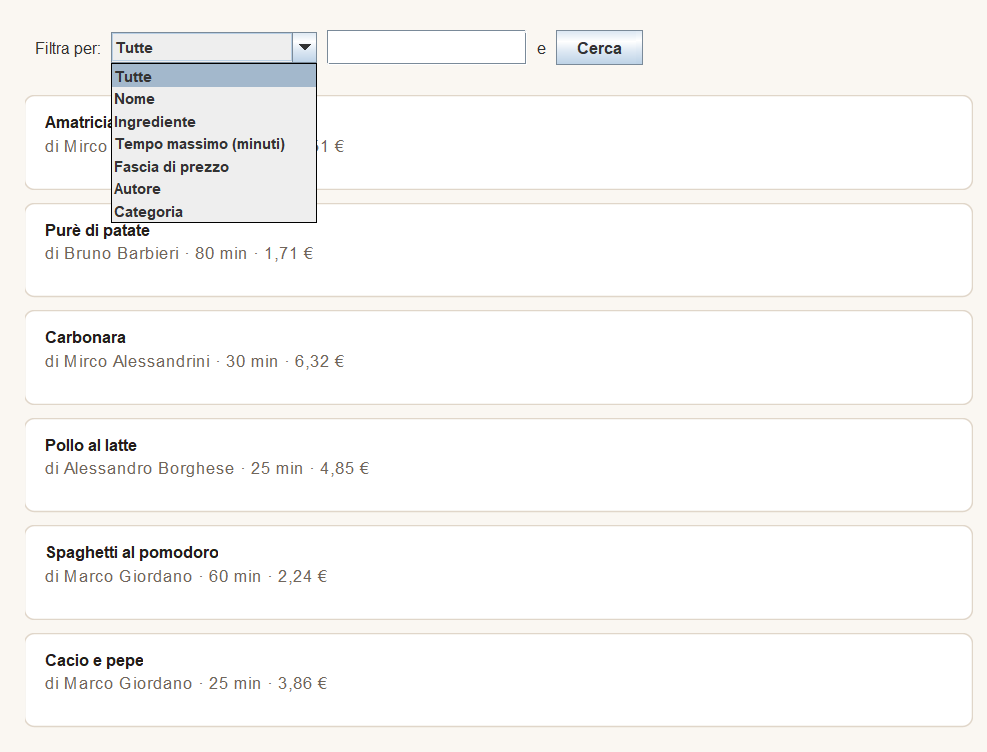
\includegraphics[width=0.8\textwidth]{images/filtro.png}
    \caption{Catalogo ricette con filtro.}
    \label{fig:filtro}
\end{figure}

\begin{figure}[H]
    \centering
    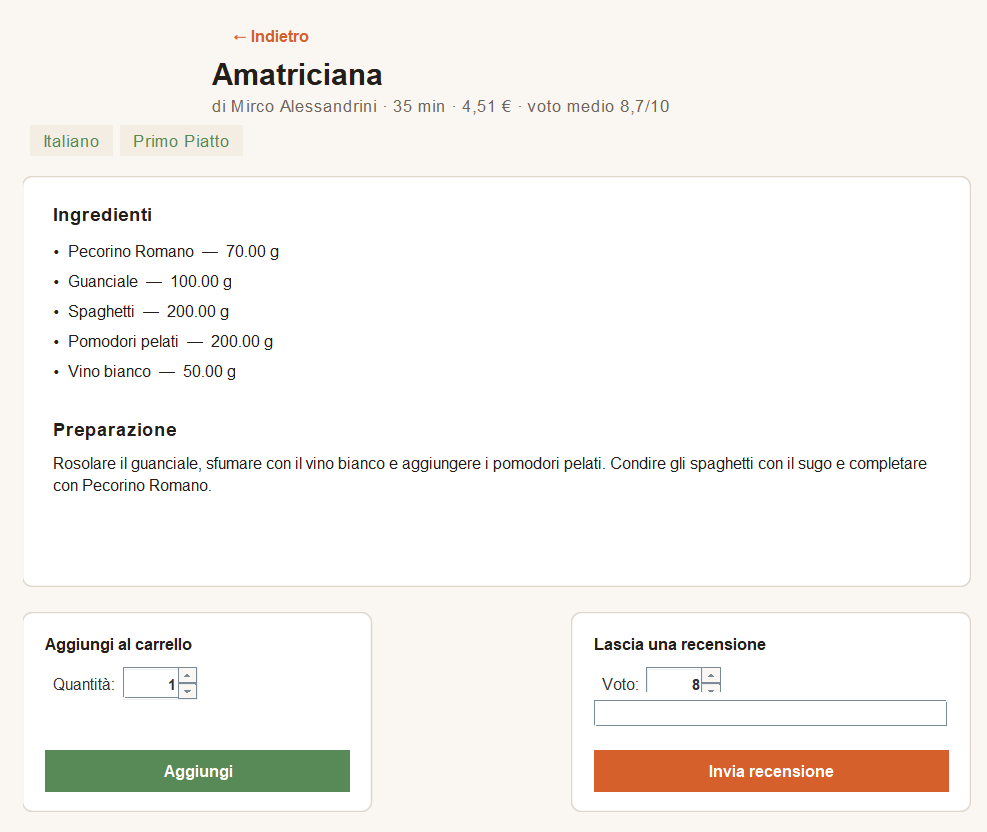
\includegraphics[width=0.8\textwidth]{images/dettaglio_ricetta.png}
    \caption{Schermata di dettaglio di una ricetta.}
    \label{fig:dett}
\end{figure}

\subsection{Pubblicazione di una nuova ricetta}

La sezione "Pubblica ricetta" presenta un form articolato in tre parti: dati generali (nome, tempo di preparazione, testo della preparazione), selezione dinamica degli ingredienti con relativa quantità in grammi (con possibilità di aggiungere e rimuovere righe prima di confermare), e selezione multipla delle categorie di appartenenza.\\
Al salvataggio, tutte le informazioni vengono registrate in un'unica operazione atomica.

\begin{figure}[H]
    \centering
    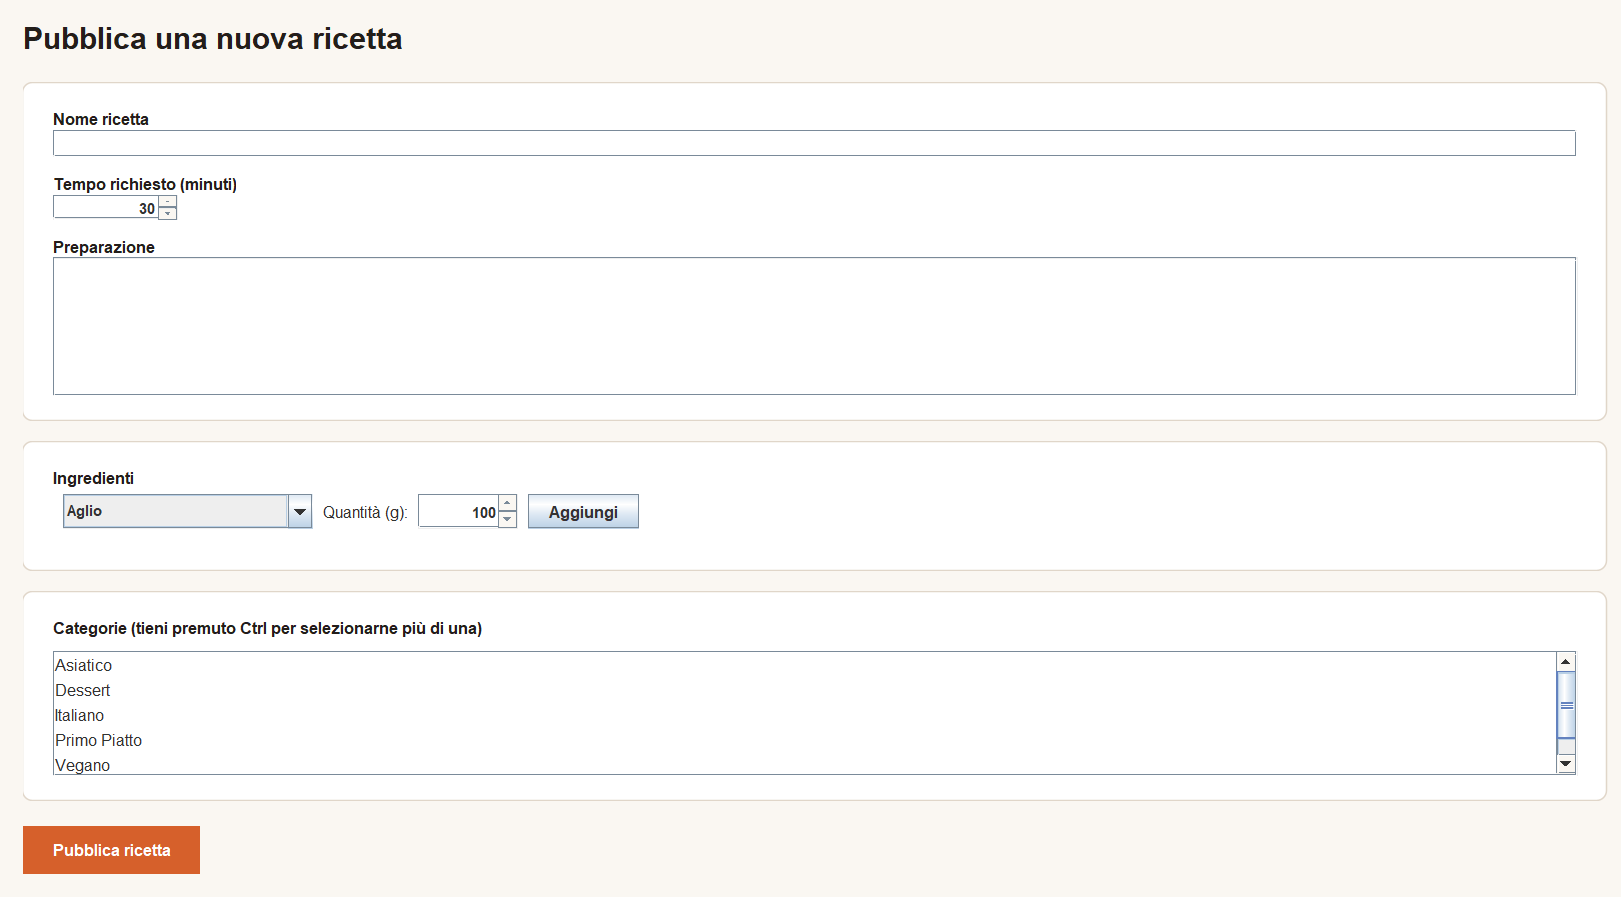
\includegraphics[width=1\textwidth]{images/pubblicazione_ricetta.png}
    \caption{Schermata di pubblicazione di una ricetta.}
    \label{fig:pubb}
\end{figure}

\subsection{Vantaggi attivi}

La sezione "Vantaggi attivi" elenca gli sconti attualmente validi, con il nome della promozione, la categoria interessata, l'intervallo di numero di ingredienti a cui si applica lo sconto, il periodo di validità e la percentuale di riduzione applicata.

\begin{figure}[H]
    \centering
    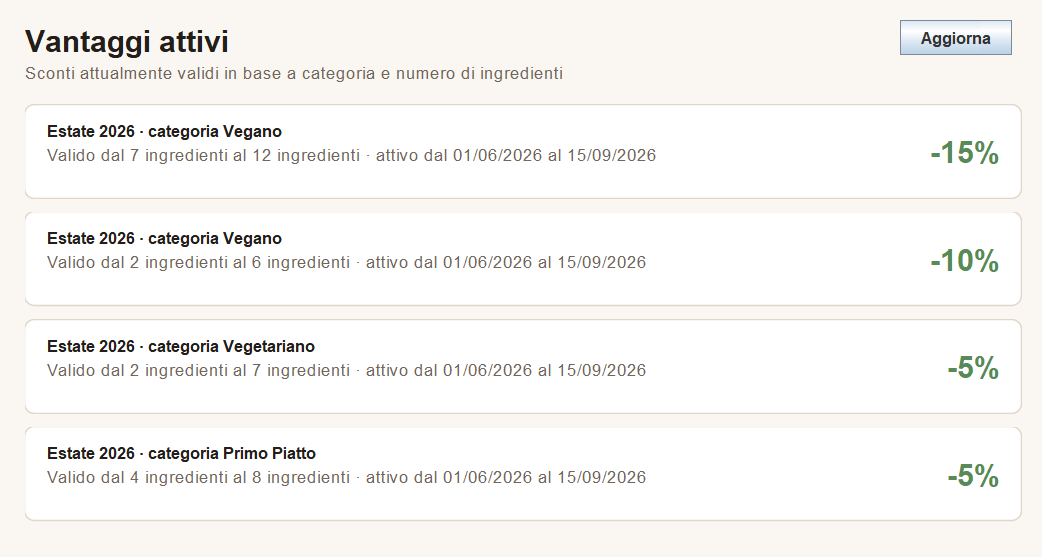
\includegraphics[width=1\textwidth]{images/vantaggi.png}
    \caption{Schermata di visualizzazione vantaggi.}
    \label{fig:vantaggi}
\end{figure}

\subsection{Carrello e conferma ordine}

Il carrello raccoglie le ricette aggiunte dall'utente durante la navigazione nel catalogo, mostrando quantità e prezzo unitario di ciascuna riga, un totale stimato e un campo per eventuali note.\\
La conferma dell'ordine applica lo sconto migliore disponibile per ciascuna ricetta al momento dell'acquisto e registra l'intero ordine in un'unica transazione.

\begin{figure}[H]
    \centering
    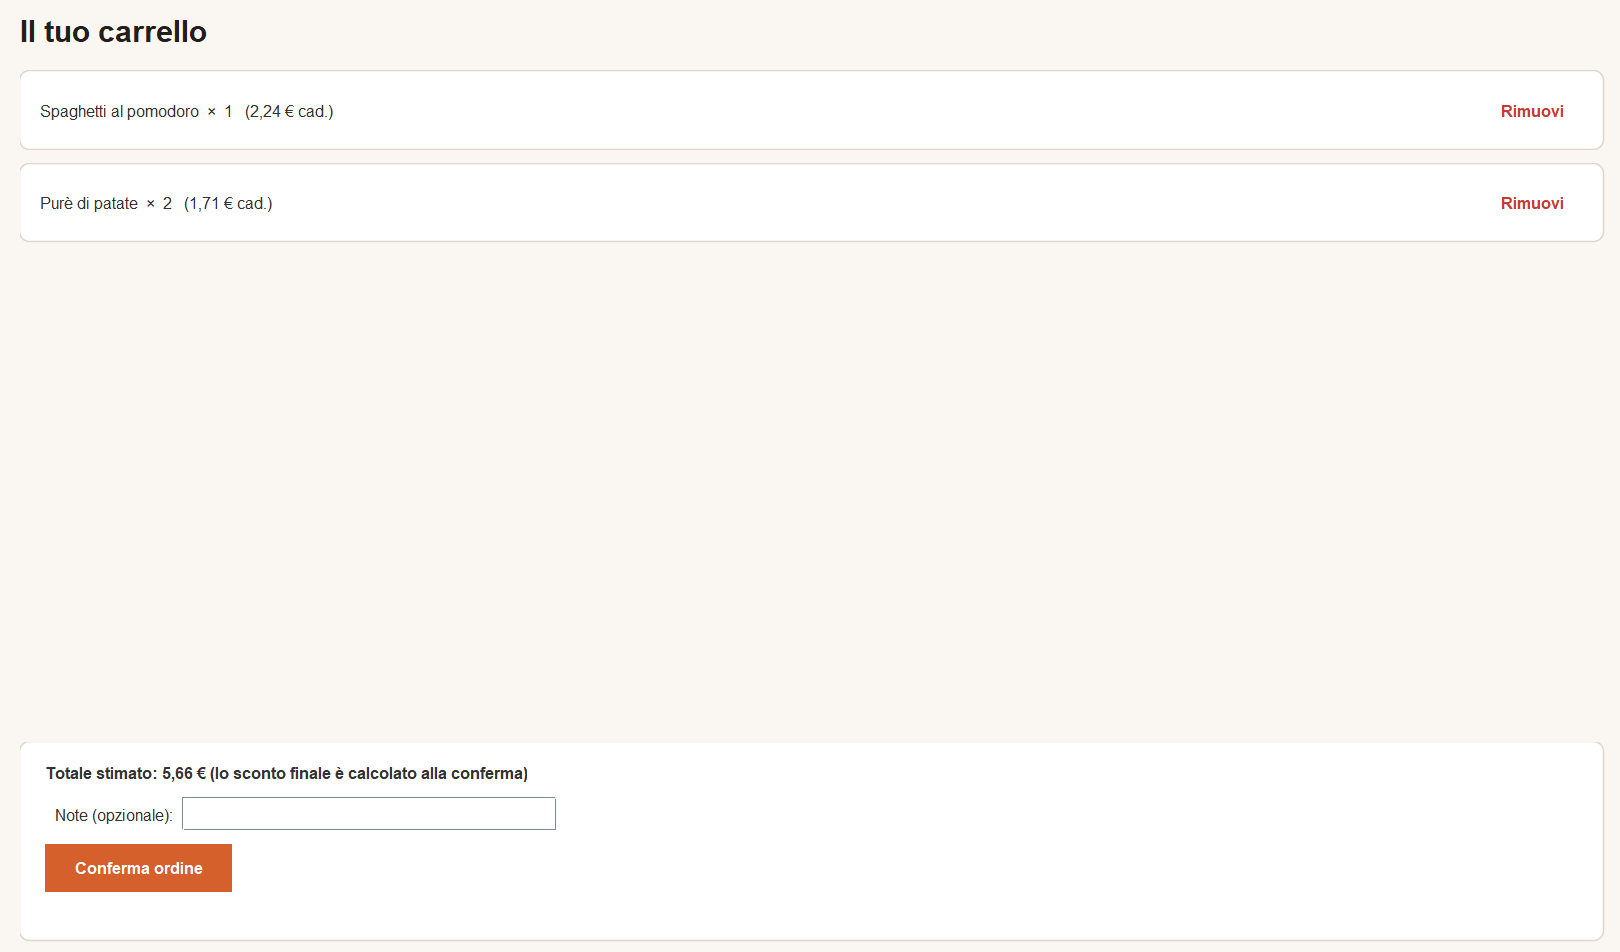
\includegraphics[width=1\textwidth]{images/carrello.png}
    \caption{Schermata di visualizzazione carrello e conferma ordine.}
    \label{fig:carrello}
\end{figure}

\subsection{Storico ordini}

Lo storico ordini raggruppa le righe di dettaglio per singolo ordine, mostrando la data, un riferimento numerico discreto, l'elenco delle ricette acquistate con relativo sconto applicato (se presente) e il totale calcolato per ciascun ordine.

\begin{figure}[H]
    \centering
    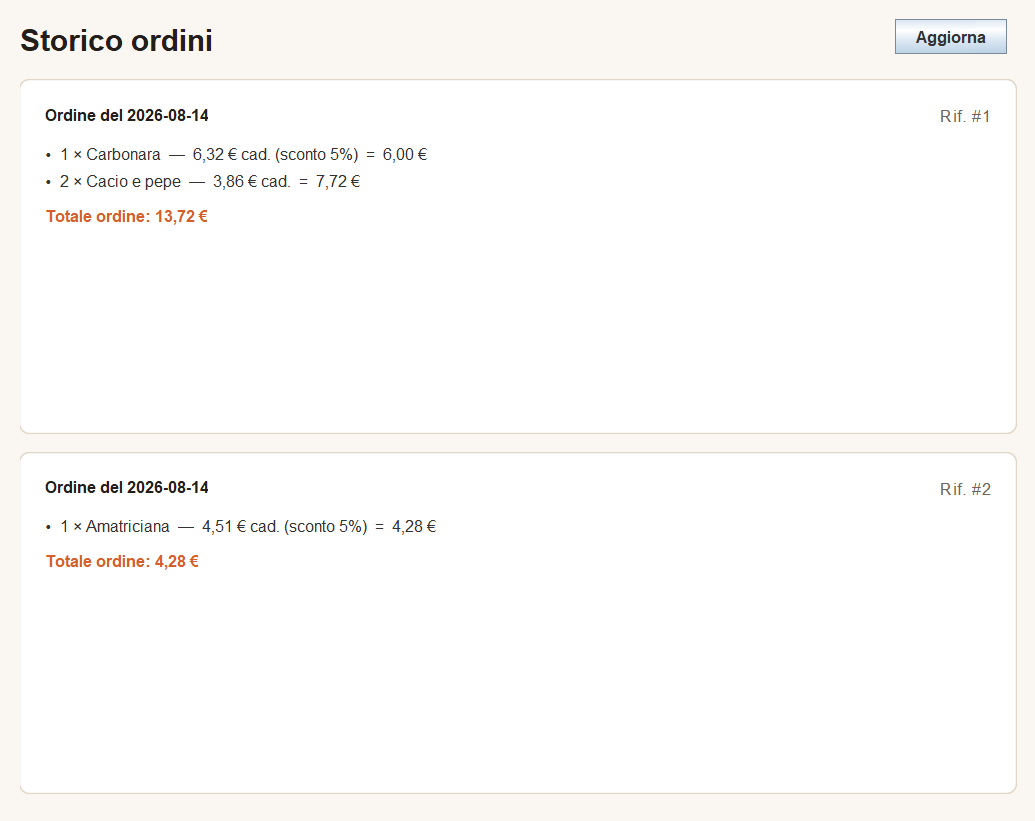
\includegraphics[width=0.8\textwidth]{images/storico_ordini.png}
    \caption{Schermata di visualizzazione storico degli ordini.}
    \label{fig:storico}
\end{figure}

\subsection{Classifiche}

La sezione "Classifiche" organizza in quattro schede le statistiche descrittive dell'applicazione: le ricette con il voto medio più alto, gli utenti con il rating medio più alto sulle proprie ricette, le ricette più ordinate e le categorie più ordinate.\\
Le righe relative a singole ricette sono cliccabili e aprono lo stesso dettaglio raggiungibile dal catalogo.

\begin{figure}[H]
    \centering
    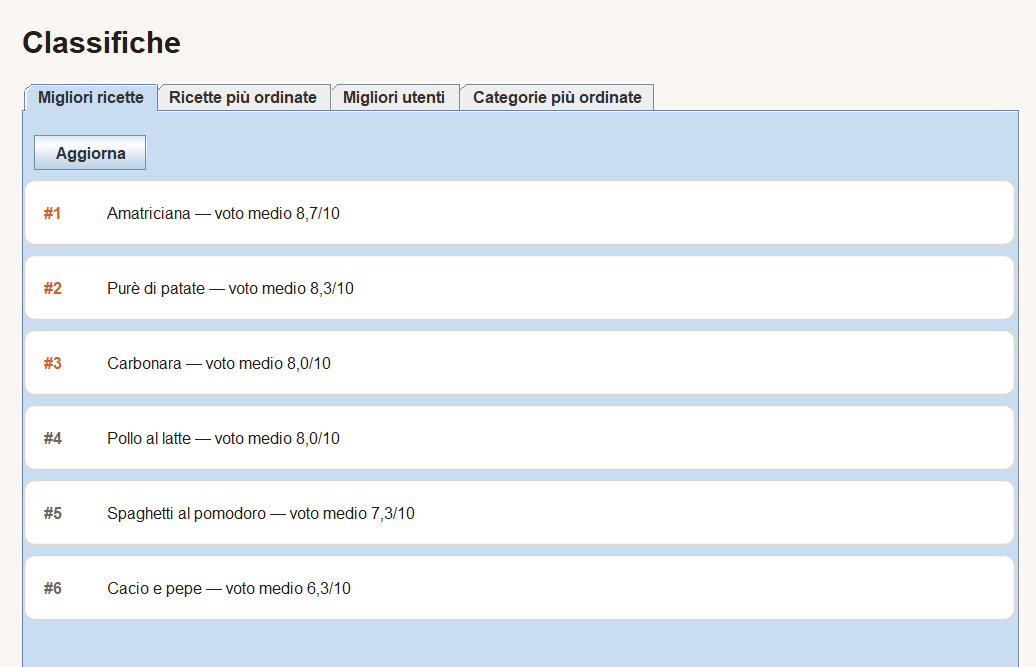
\includegraphics[width=0.8\textwidth]{images/classifiche.png}
    \caption{Schermata di visualizzazione migliori ricette in base alle recensioni.}
    \label{fig:classifiche}
\end{figure}

\subsection{Pannello amministratore}

Visibile esclusivamente agli utenti con ruolo ADMIN, il pannello amministratore è organizzato in cinque schede: gestione ingredienti (creazione e modifica), gestione categorie, gestione di promozioni e sconti, esecuzione dell'operazione di rimozione degli utenti incoerenti (con richiesta di conferma esplicita), e una sezione di report che espone in forma tabellare le tre viste SQL definite nello schema fisico: fatturato giornaliero, fatturato per ricetta e recensioni negative recenti.

\begin{figure}[H]
    \centering
    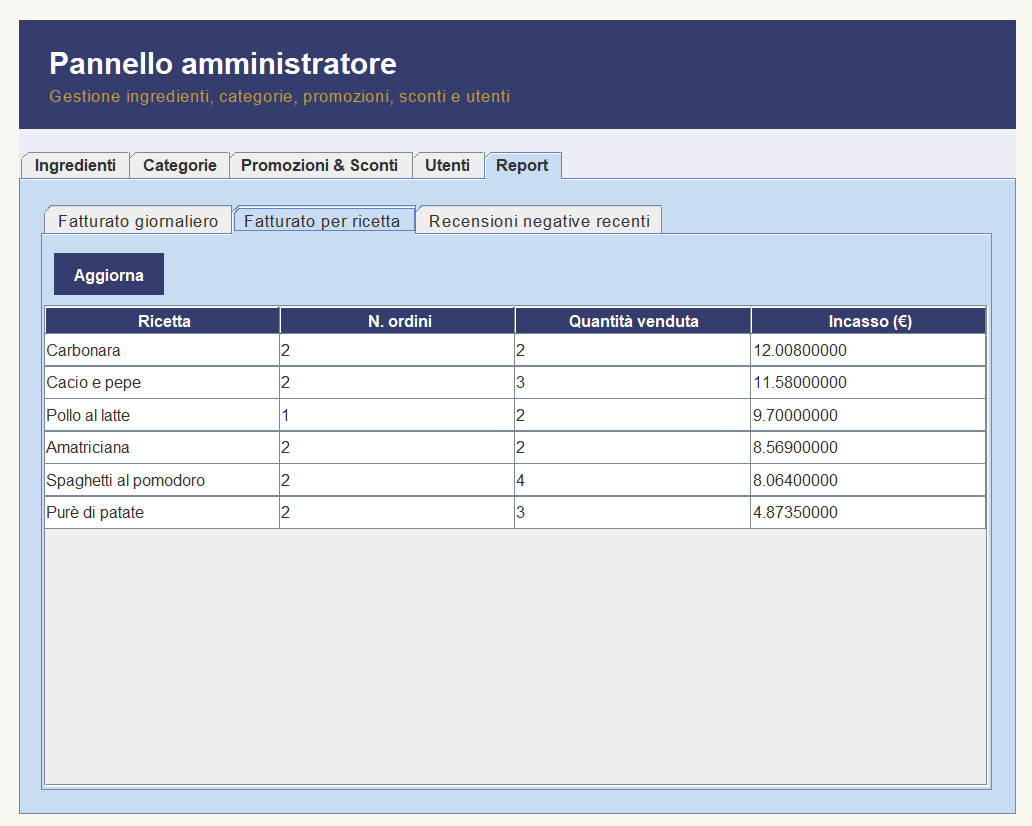
\includegraphics[width=0.8\textwidth]{images/admin.png}
    \caption{Schermata di visualizzazione report lato amministratore.}
    \label{fig:admin}
\end{figure}




